\section[Расчётная часть]{РАСЧЁТНАЯ ЧАСТЬ}

\subsection{Описание комплекса технических средств системы}

Предполагается, что проектируемое приложение будет использоваться
на мобильных устройствах под управлением операционной системы Android
версии не ниже 4.1.

Для полноценной работы приложения требуется наличие фотокамеры.

\subsection{Организация работы системы}

Рассмотрим несколько диаграмм, разработанных по методологиям IDEF0 и IDEF3,
описывающих работу проектируемого приложения.

% main
На рисунке~\ref{fig:idef0_main} представлена диаграмма декомпозиции
верхнего уровня.

\begin{figure}[h!]
  \centering
  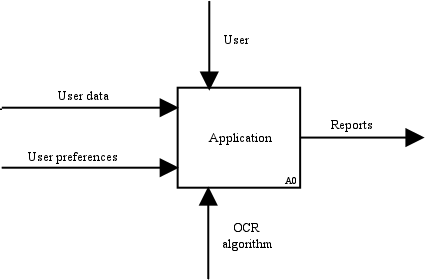
\includegraphics[width=130mm]{pic/idef0_main}
  \caption{Диаграмма декомпозиции \\ верхнего уровня}
  \label{fig:idef0_main}
\end{figure}

Из этого рисунка видно, что входом системы служат финансовые данные пользователя,
а также его личные предпочтения,
результатом работы системы являются финансовые отчёты,
роль механизма выполняет алгоритм распознавания изображений (OCR),
а управление осуществляет пользователь приложения.

\pagebreak
% application
На рисунке~\ref{fig:idef0_app} представлена диаграмма декомпозиции
приложения.

\begin{figure}[h!]
  \centering
  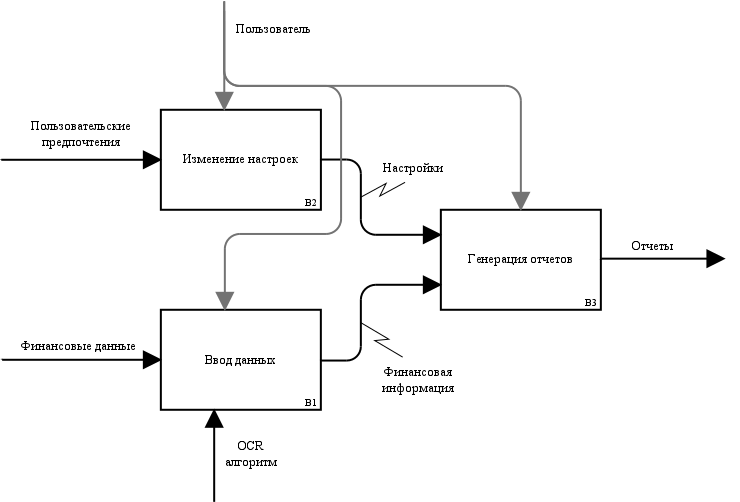
\includegraphics[width=150mm]{pic/idef0_app}
  \caption{Диаграмма декомпозиции приложения}
  \label{fig:idef0_app}
\end{figure}

Работу приложения можно разделить на следующие этапы:
\begin{itemize}
\item настройка параметров приложения;
\item ввод финансовых данных;
\item генерация отчётов на основании данных и настроек.
\end{itemize}

Входом для блока <<Изменение настроек>> являются пользовательские
предпочтения, а выходом --- настройки, сохраненные в системе.

Финансовые данные, обрабатываемые в блоке <<Ввод данных>>
с использованием алгоритма распознавания изображений,
преобразуются в структурированную финансовую информацию.

Финансовая информация и настройки приложения определяют содержание
отчётов, производимых в блоке <<Генерация отчётов>>.

\pagebreak
% settings
Рассмотрим более подробно процесс выбора настроек приложения,
представленный на рисунке~\ref{fig:idef3_settings}.

\begin{figure}[h!]
  \centering
  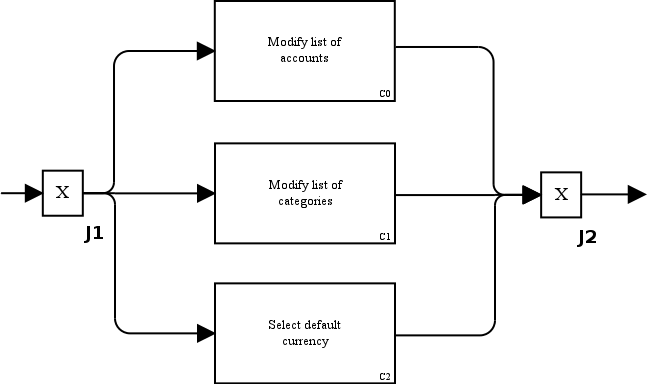
\includegraphics[width=150mm]{pic/idef3_settings}
  \caption{Диаграмма выбора настроек приложения}
  \label{fig:idef3_settings}
\end{figure}

В соответствии с ним, пользователь имеет возможность
добавить или удалить финансовый счёт,
добавить или удалить категорию учета денежных средств,
а также выбрать валюты ввода и представления финансовых
данных по умолчанию.

\pagebreak
% input
Рассмотрим процесс ввода данных,
представленный на рисунке~\ref{fig:idef3_input}.

\begin{figure}[h!]
  \centering
  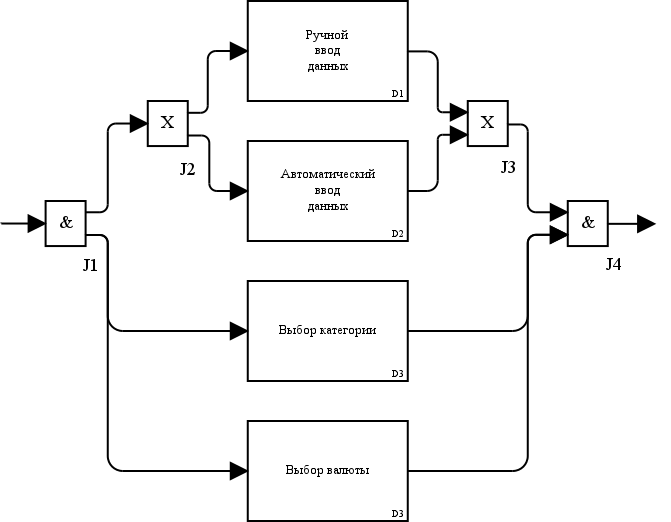
\includegraphics[width=150mm]{pic/idef3_input}
  \caption{Диаграмма процесса ввода данных}
  \label{fig:idef3_input}
\end{figure}

В соответствии с ним, пользователь может вводить числовые данные
вручную, либо с помощью фотокамеры; выбирать выбрать категорию учета,
а также дату ввода.


\pagebreak
% input
Наконец, рассмотрим процесс получения финансовых отчётов,
представленный на рисунке~\ref{fig:idef3_reports}.

\begin{figure}[h!]
  \centering
  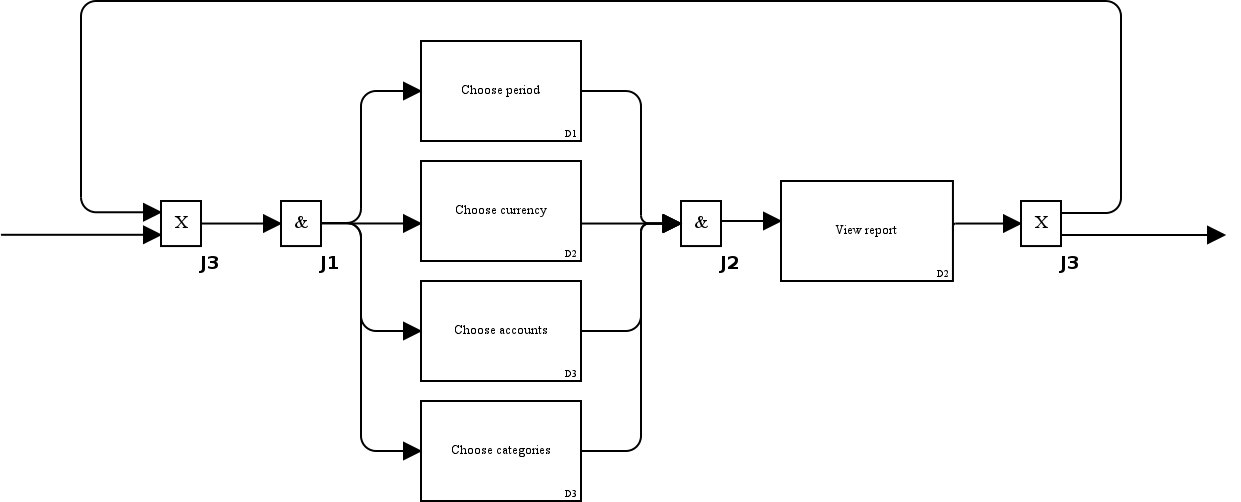
\includegraphics[width=150mm]{pic/idef3_reports}
  \caption{Диаграмма процесса получения отчёта}
  \label{fig:idef3_reports}
\end{figure}

В соответствии с представленной диаграммой, для получения
финансового отчёта пользователь должен выбрать финансовый счёт,
категории учета, а также учетный период.
На основании этих предпочтений пользователя, а также информации
об изменении финансового состояния пользователя,
хранящейся в базе данных, система предоставит требуемый финансовый отчёт.

\pagebreak
\subsection{Пользовательский интерфейс системы}

В данном разделе будет рассмотрен дизайн системы с точки зрения
конечного пользователя.

Приложения, разрабатываемые для мобильных платформ, можно разделить
на <<экраны>> --- различные части приложения, выполняющие некоторую
определенную роль.

Примерами таких <<экранов>> для проектируемого приложения являются:
\begin{itemize}
\item <<главный>> экран;
\item экран ввода данных;
\item экран вывода состояния счёта.
\end{itemize}

На рисунке~\ref{fig:screen_main} представлен главный экран приложения.

\begin{figure}[h!]
  \centering
  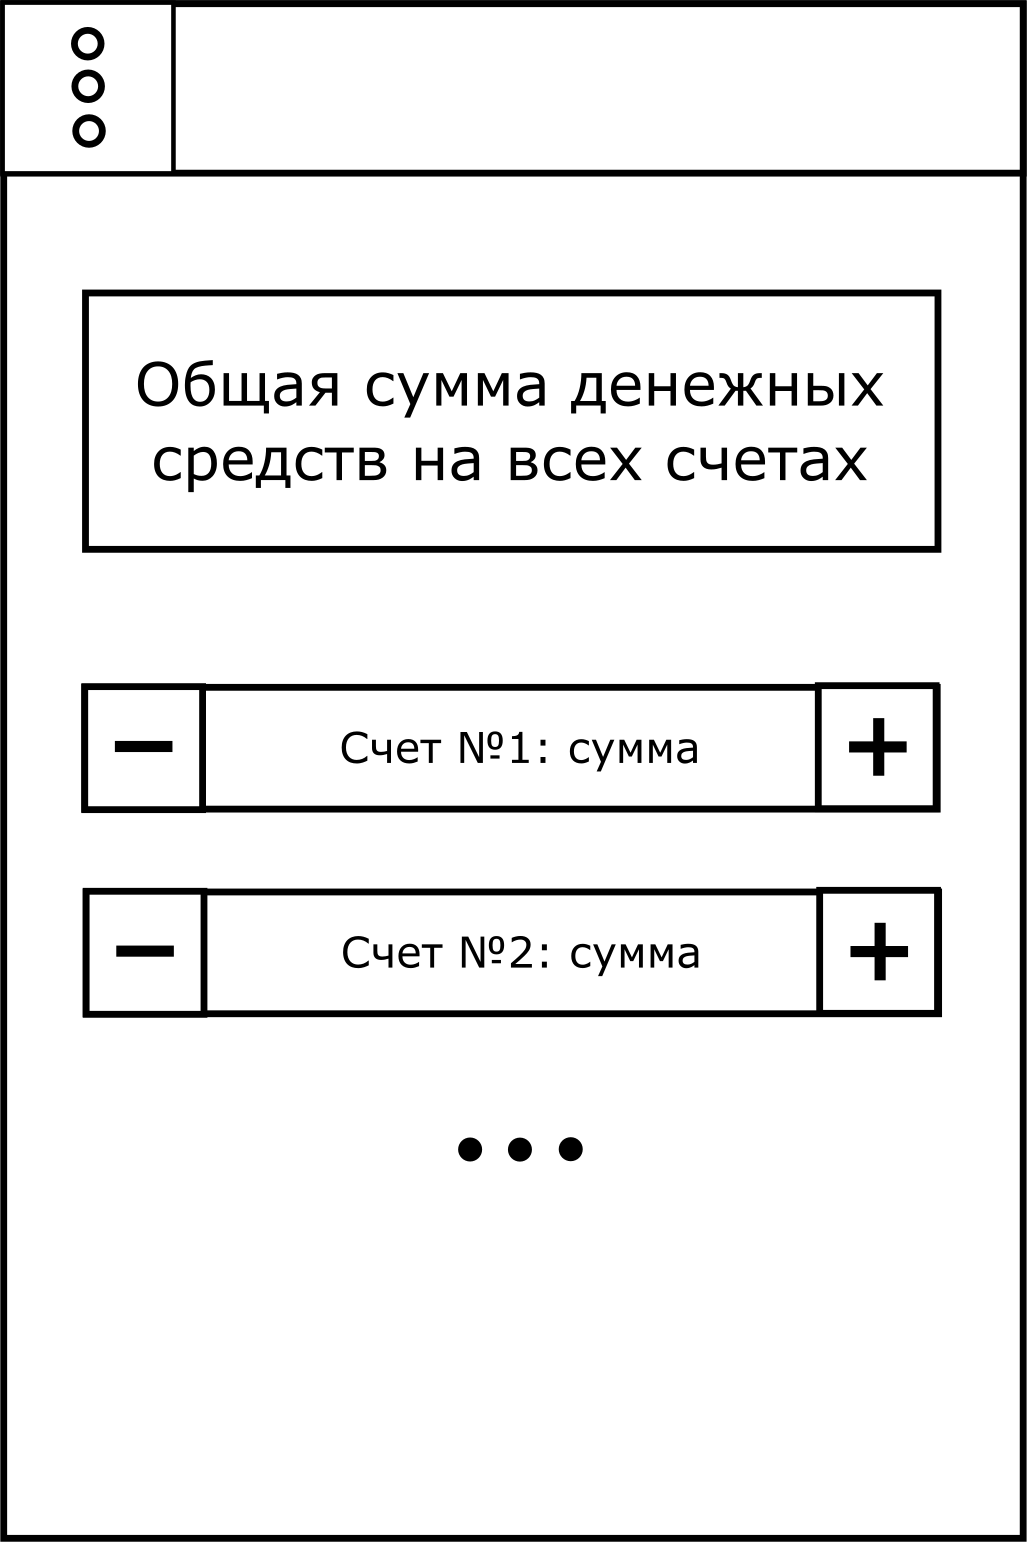
\includegraphics[width=75mm]{pic/screen_main}
  \caption{Главный экран приложения}
  \label{fig:screen_main}
\end{figure}

Он отображает общий баланс денежных средств пользователя,
а также предоставляет возможность ввода финансовых данных для
выбранного счёта (<<Работа>>, <<Стипендия>>).

По нажатию на значение состояния счёта производится переход на
экран вывода состояния счёта.

На рисунке~\ref{fig:screen_input} представлен макет экрана ввода данных.

\begin{figure}[h!]
  \centering
  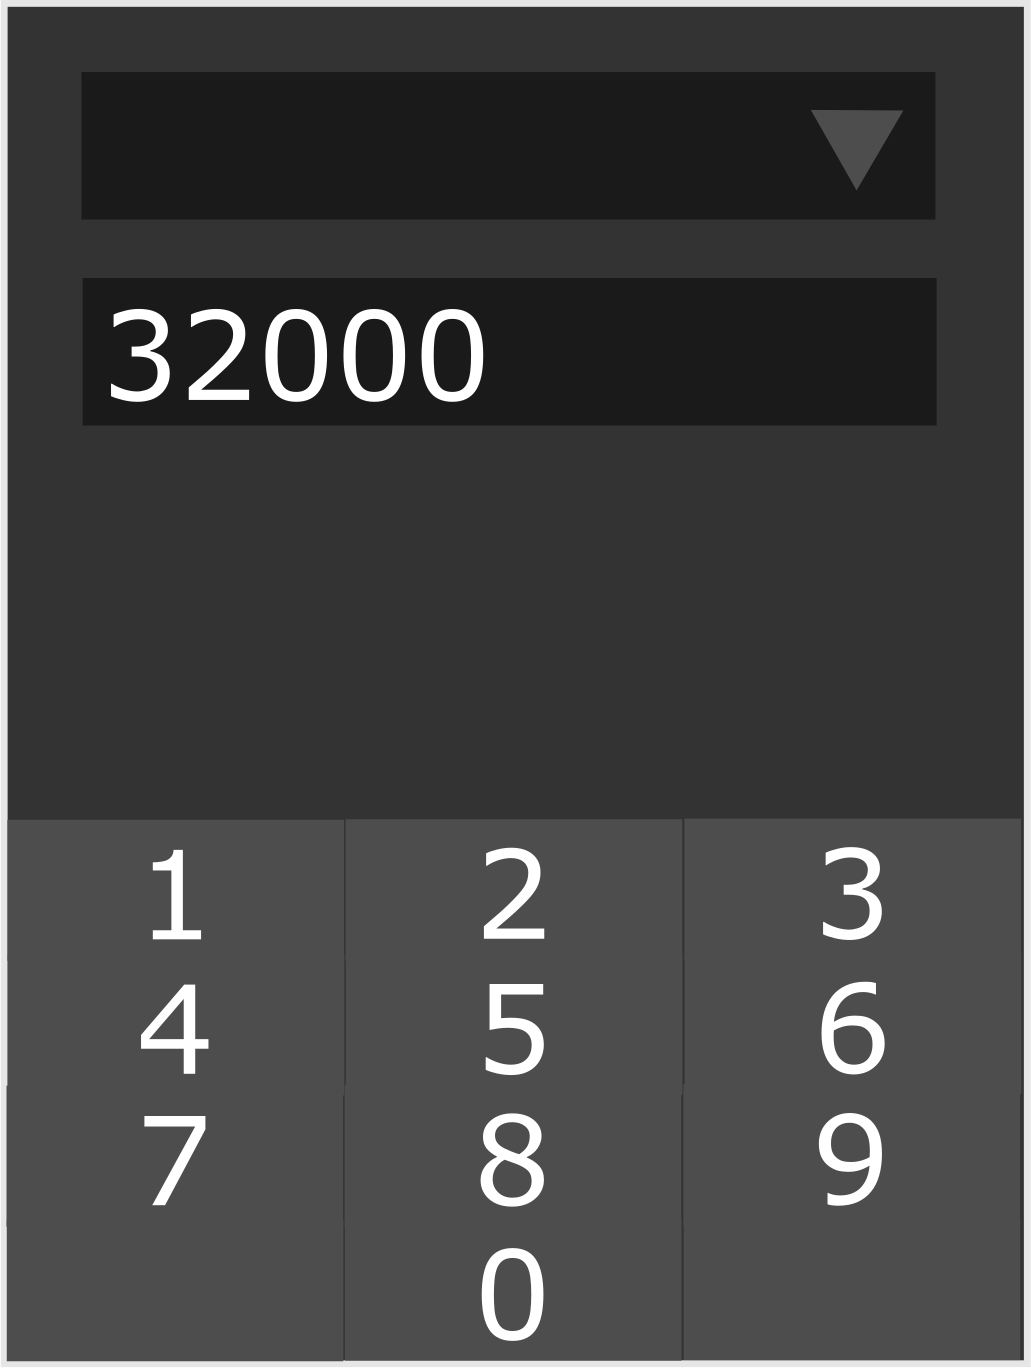
\includegraphics[width=55mm]{pic/screen_input}
  \caption{Экран ввода данных}
  \label{fig:screen_input}
\end{figure}

На этом экране пользователь может вручную указать требуемую сумму,
а также выбрать категорию учета.

На рисунке~\ref{fig:screen_account} представлен экран состояния
счёта пользователя.

\begin{figure}[h!]
  \centering
  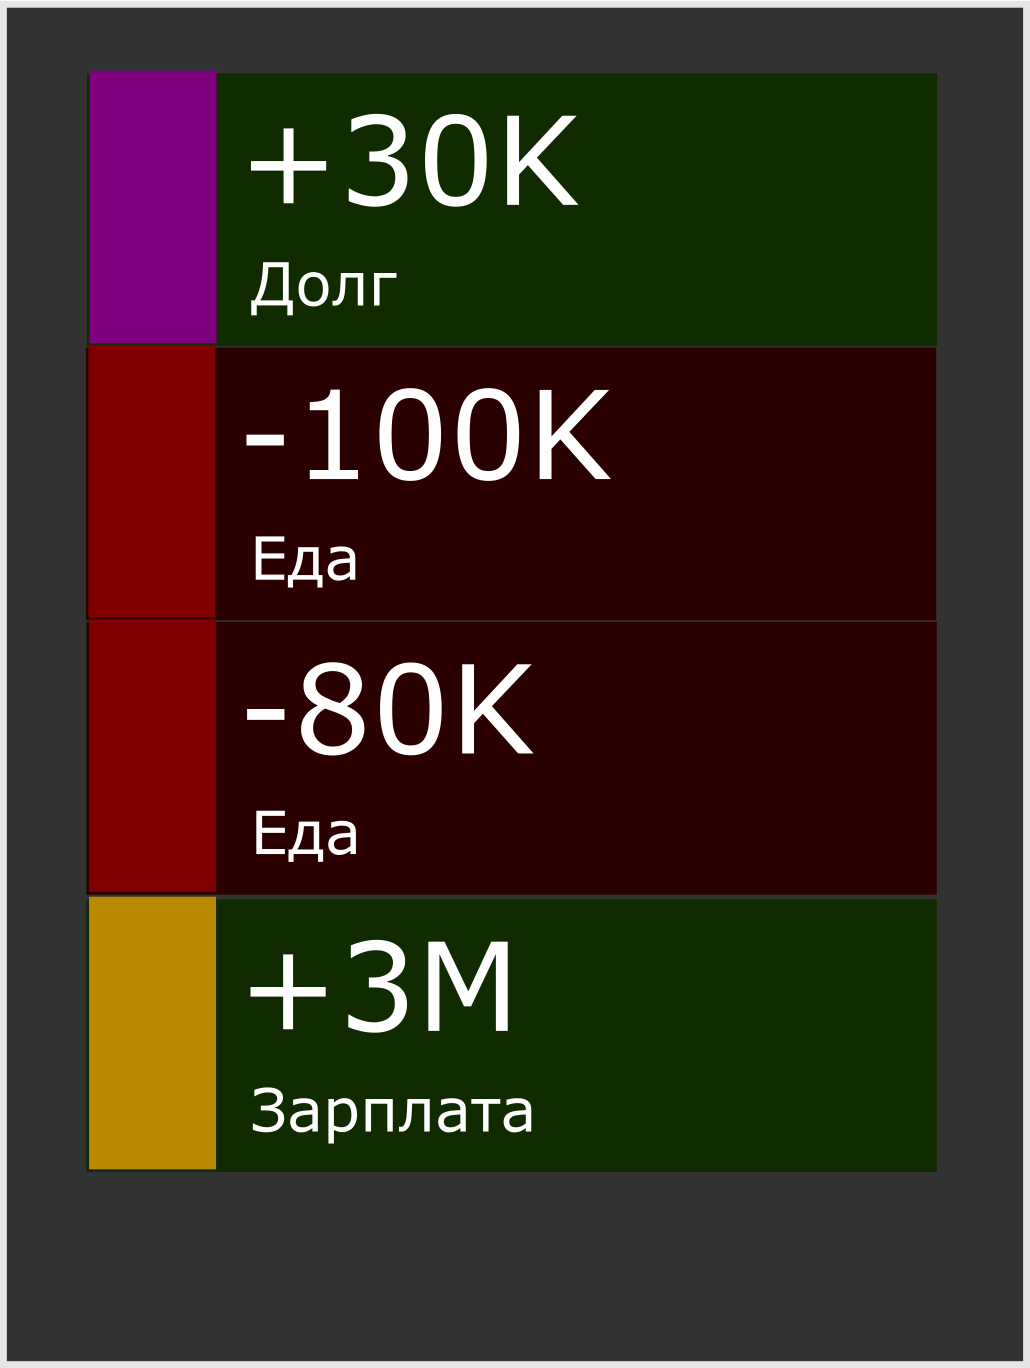
\includegraphics[width=55mm]{pic/screen_account}
  \caption{Экран вывода состояния счёта}
  \label{fig:screen_account}
\end{figure}

Он содержит список записей об изменении состояния счёта пользователя.
Каждая запись содержит значение изменения состояния счёта, категорию
учета, отмеченную названием, а также условным цветом заливки (слева).